% This is samplepaper.tex, a sample chapter demonstrating the
% LLNCS macro package for Springer Computer Science proceedings;
% Version 2.21 of 2022/01/12
%
\documentclass[runningheads]{llncs}
%
\usepackage[T1]{fontenc}
% T1 fonts will be used to generate the final print and online PDFs,
% so please use T1 fonts in your manuscript whenever possible.
% Other font encondings may result in incorrect characters.
%
\usepackage{graphicx}
% Used for displaying a sample figure. If possible, figure files should
% be included in EPS format.
%
% If you use the hyperref package, please uncomment the following two lines
% to display URLs in blue roman font according to Springer's eBook style:
%\usepackage{color}
%\renewcommand\UrlFont{\color{blue}\rmfamily}
%\urlstyle{rm}
%

\usepackage[colorlinks=true,linkcolor=blue,citecolor=blue]{hyperref}
\usepackage{amsmath}
\usepackage{multirow}

\begin{document}
%
\title{Analyzing ESG-washing Risk: A case study in Vietnamese Banking Annual Reports}
%
\titlerunning{ESG-washing Risk in Vietnamese Banks}
% If the paper title is too long for the running head, you can set
% an abbreviated paper title here
%
\author{Huu Huy Pham \and Viet Anh Nguyen\thanks{Corresponding author: vietanh@vnu.edu.vn}}
%
\authorrunning{H. H. Pham and V. A. Nguyen}
% First names are abbreviated in the running head.
% If there are more than two authors, 'et al.' is used.
%
\institute{VNU University of Engineering and Technology, Hanoi, Vietnam
% \\
\email{22028237@vnu.edu.vn}, \email{vietanh@vnu.edu.vn}
}
%
\maketitle              % typeset the header of the contribution
%

\begin{abstract}
ESG disclosures have become central to corporate reporting in the banking sector, yet the rapid expansion of ESG communication has intensified concerns about ESG-washing. Existing detection approaches often rely on third-party ESG ratings, which suffer from limited coverage and reliability in emerging markets. This study proposes an NLP-driven neuro--symbolic framework that evaluates ESG-washing risk through the internal verifiability of ESG statements within banks’ annual reports. The framework integrates ESG topic classification, actionability assessment, and evidence linkage into a composite ESG-Washing Risk Index (EWRI). Experimental results show high classification accuracy and demonstrate that the proposed evidence-linking mechanism outperforms keyword-based baselines. Empirical analysis of Vietnamese banks reveals significant cross-bank differences and a temporal peak in ESG-washing risk in 2022, followed by a decline as disclosures increasingly emphasize concrete actions. The findings highlight the effectiveness of internal text-based analysis for ESG-washing detection in data-constrained emerging markets.
\keywords{ESG-washing \and Annual reports \and Banking \and NLP \and Neuro--symbolic systems}
\end{abstract}
%
%
%

\section{Introduction}
ESG disclosure has become an indispensable component of corporate reporting in the banking sector, where sustainability commitments are increasingly scrutinized by regulators, investors, and the public \cite{buchetti2025literature,lagasio2024esg}. While annual reports serve as a primary channel for communicating ESG initiatives, the growing prominence of ESG narratives has amplified the risk of ESG-washing---the practice of emphasizing favorable sustainability claims without sufficient verifiable evidence \cite{florstedt2025detecting}.

Prior research shows that ESG-washing undermines market transparency, erodes stakeholder trust, and distorts investment decision-making, thereby increasing the risk of inefficient capital allocation \cite{lagasio2024esg,florstedt2025detecting}. These risks are particularly pronounced in the banking sector, as illustrated by the 2022 controversy surrounding sustainable investment funds linked to Deutsche Bank AG \cite{lipenkova2023detecting}. Moreover, ESG disclosures have been shown to directly influence investors’ perceptions of banks’ risk management quality and institutional credibility \cite{kathan2025you}. As a result, systematic ESG-washing analysis in banking reports is of both academic and regulatory relevance.

Existing approaches to ESG-washing detection can be broadly grouped into two methodological streams. The first relies on rating-discrepancy analysis, measuring divergences between firms’ ESG disclosures and third-party ESG performance ratings \cite{su16062571,ghitti2024agency}. The second stream adopts text-based and NLP-driven methods to analyze linguistic patterns in ESG disclosures \cite{lagasio2024esg,lipenkova2023detecting,zhao2023detecting}. Although these methods offer greater scalability, they often lack mechanisms for verifying whether ESG statements are internally supported by concrete evidence.

To address these limitations, this study proposes an NLP-based neuro--symbolic framework for ESG-washing analysis in banks’ annual reports, in which ESG-washing risk is assessed through the internal verifiability of ESG disclosures. Rather than benchmarking disclosures against external ESG performance metrics, the framework evaluates the extent to which ESG statements are substantiated by concrete, traceable actions and evidence within the same document. These assessments are aggregated into a report-level ESG-Washing Risk Index (EWRI).

This study makes three main contributions. First, it introduces an internal-verifiability perspective for ESG-washing analysis, shifting the focus from external rating discrepancies to evidence-based evaluation within corporate disclosures. Second, it develops a scalable NLP-based framework that enables systematic and graded assessment of ESG-washing risk beyond binary classification. Third, it provides empirical evidence from the Vietnamese banking sector, thereby extending ESG and NLP research to data-constrained emerging markets.

The remainder of this paper is organized as follows. Section~2 reviews related work on ESG-washing and existing measurement approaches. Section~3 describes the proposed methodological framework and the construction of EWRI. Section~4 presents and discusses the empirical results. Section~5 concludes the paper and outlines directions for future research.


%
%
%
\section{Related Works}
ESG disclosure has evolved from voluntary communication to a core component of mandatory reporting frameworks, particularly in jurisdictions such as the European Union \cite{lagasio2024esg}. In the banking sector, ESG reporting is closely linked to risk management, governance quality, and capital allocation, especially in the context of green finance and sustainable lending. As ESG reporting expands, the literature has increasingly highlighted ESG-washing as a critical concern, referring to situations in which firms emphasize positive ESG claims while providing limited evidence of substantive actions \cite{lagasio2024esg}. Prior studies document that ESG-washing undermines stakeholder trust and distorts information environments, with particularly severe implications for the banking industry.

Recent studies have sought to develop quantitative and semi-automated approaches for detecting ESG-washing in corporate reports by leveraging natural language processing (NLP), sentiment analysis, and composite indicators. While these approaches provide important methodological contributions, they also exhibit notable limitations related to language coverage, data availability, and the interpretability of analytical outcomes.

Florstedt and Fahlbusch (2025) propose a hybrid NLP framework to identify ESG-related “cheap talk” in corporate disclosures. Their approach combines sentiment analysis using VADER, linguistic specificity assessment via ClimateBERT, and internal evidence retrieval based on Sentence-BERT. Their results show that highly positive yet vague ESG statements lacking internal support are strongly associated with elevated ESG-washing risk. However, the framework is primarily designed for English texts and does not incorporate explicit logical reasoning to systematically validate extracted evidence \cite{florstedt2025detecting}.

Lipenkova et al. (2023) conduct a comparative analysis of ESG disclosures by German firms against external information sources such as news media and non-governmental organizations. By employing sentence embeddings and transformer-based models, the study aims to identify discrepancies between internally reported ESG claims and externally observed practices. The findings indicate that firms exhibiting overly positive self-assessments while receiving contradictory external coverage are more likely to engage in ESG-washing \cite{lipenkova2023detecting}. However, this approach relies heavily on reliable external data sources, which are often scarce or fragmented in emerging markets such as Vietnam, where ESG-focused journalism and independent monitoring remain limited.

Lagasio (2024) proposes a text-based quantitative approach combining TF–IDF, Latent Dirichlet Allocation (LDA), and sentiment analysis to construct an ESG-washing Severity Index (ESGSI). The index captures the divergence between positive ESG language and the substantive depth of ESG-related disclosures, with higher values indicating greater ESG-washing risk. Applied to 749 firms, the ESGSI reveals substantial variation across industries and regions \cite{lagasio2024esg}. However, the index focuses on stylistic and topical imbalances and does not assess the factual accuracy or internal consistency of ESG claims, making it potentially sensitive to promotional reporting styles.

Taken together, these studies demonstrate the growing potential of linguistic analysis, sentiment modeling, and language-based representations for ESG-washing detection. However, several limitations remain. First, most existing approaches are designed for English-language corpora and offer limited applicability to under-resourced languages such as Vietnamese. Second, many methods depend on external ESG ratings or third-party information sources, which are often unavailable or unreliable in developing markets. Third, few systems incorporate cross-sentence reasoning or logical consistency checks, increasing the risk of misclassification when ESG statements involve implicit assumptions or contextual dependencies. These limitations highlight the need for ESG-washing detection frameworks that support deeper semantic analysis, internal content verification, and contextual understanding of ESG-related claims.

%
%
%
\section{Methodology}
The framework of this study is designed as an analytical pipeline, as illustrated in Fig.~\ref{framework}.

\begin{figure}[!t]
\centering
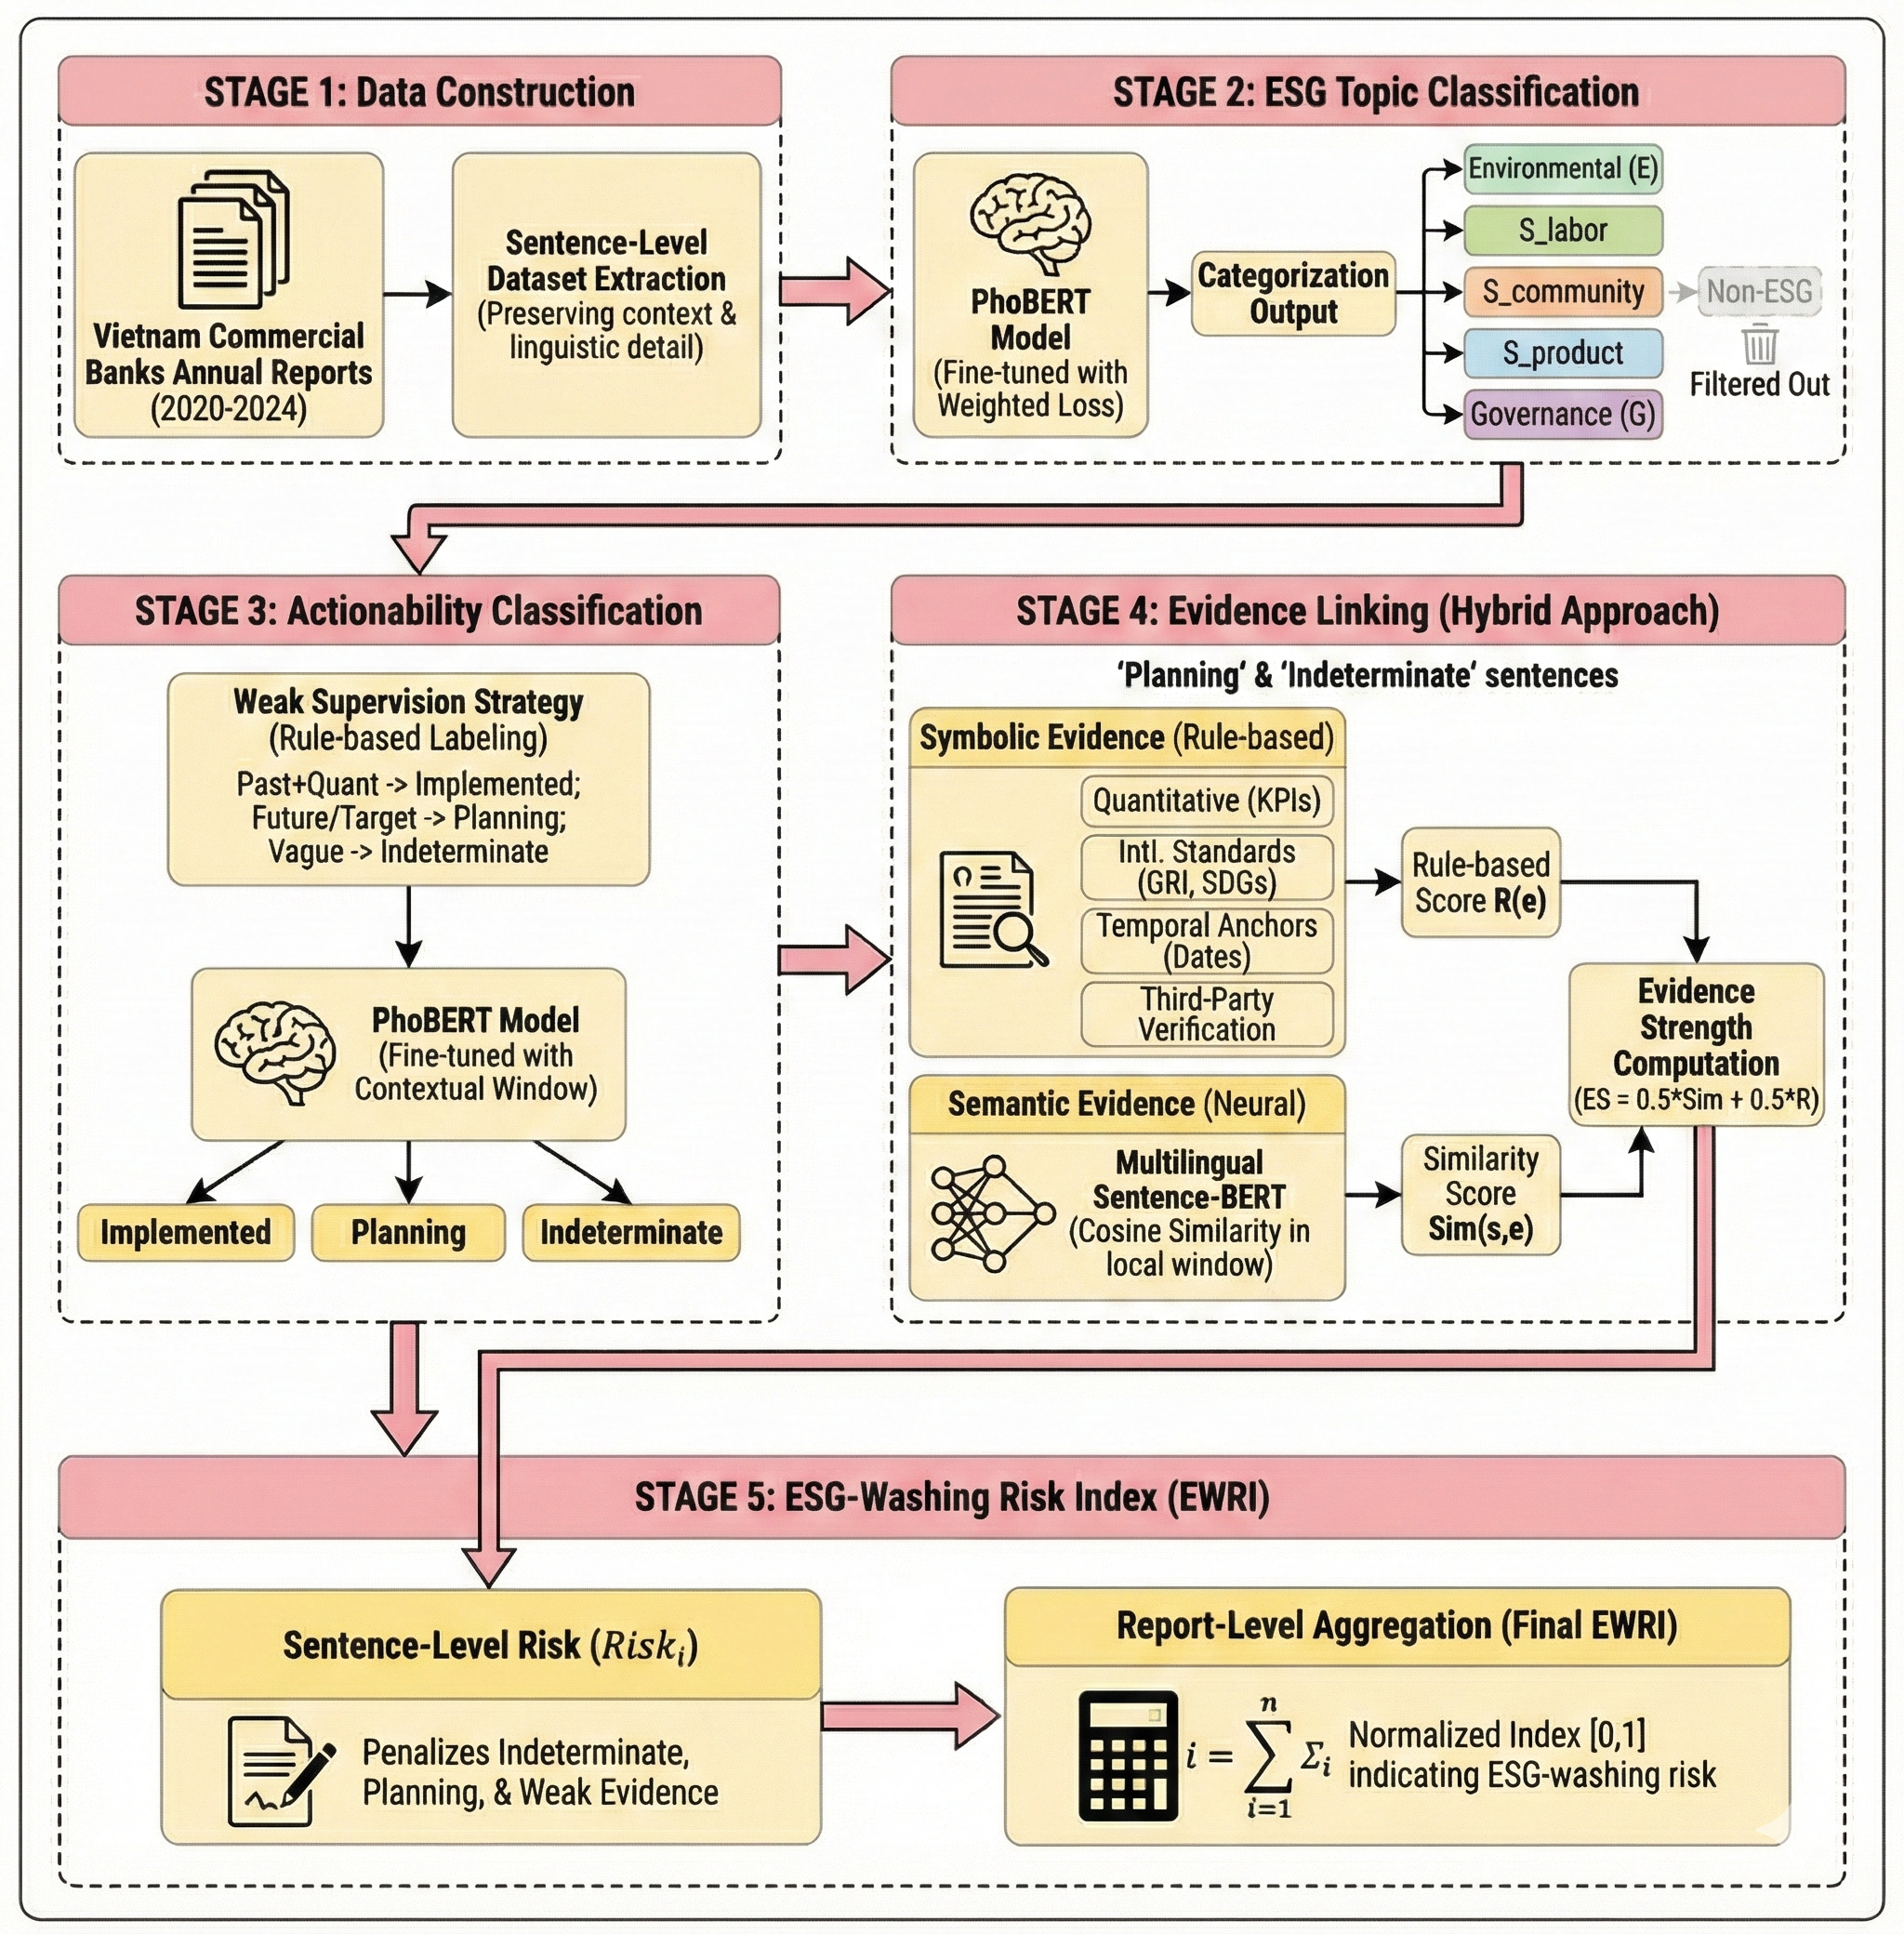
\includegraphics[width=0.7\textwidth]{figures/framework.png}
\caption{Overview of the proposed ESG-washing detection framework, designed as a five-stage analytical pipeline comprising data construction, ESG topic classification, actionability classification of ESG statements, evidence detection and linking, and EWRI computation.} \label{framework}
\end{figure}

\subsection{Data Construction}
The dataset is constructed at the sentence level using ESG-related statements extracted from the annual reports of selected commercial banks in Vietnam (2020--2024). This design enables fine-grained analysis by preserving linguistic detail, contextual dependencies, and temporal structure, which are critical for identifying discrepancies between ESG commitments and substantive actions that may be obscured in document-level aggregation.

\subsection{ESG Topic Classification}
To isolate ESG-relevant content, each sentence is first classified into one of the following categories: Non-ESG, Environmental (E), S\_labor, S\_community, S\_product, Governance (G). This step filters out non-ESG content and assigns ESG-relevant sentences to fine-grained thematic categories, enabling structured analysis across different ESG dimensions.

For this task, the PhoBERT language model is fine-tuned to perform ESG topic classification at the sentence level. PhoBERT is selected due to its strong performance on Vietnamese natural language understanding tasks and its suitability for domain-specific fine-tuning. Class imbalance in the training data is addressed through a weighted loss function, ensuring that minority classes are not dominated by more prevalent categories during model optimization.

The output of this stage is a subset of sentences identified as ESG-related, each assigned to a specific thematic category. Sentences classified as Non-ESG are excluded from further processing, allowing subsequent stages of the pipeline to focus exclusively on content that is substantively relevant to ESG analysis.

\subsection{Actionability Classification}
\subsubsection{Definition of Actionability Levels}
Each ESG sentence is further assessed in terms of its level of actionability, which reflects the extent to which the sentence describes concrete ESG-related actions rather than abstract intentions or generic statements. We define three levels of actionability: (i) \emph{Implemented}---completed or ongoing ESG actions, often referring to past activities or measurable outcomes; (ii) \emph{Planning}---future-oriented commitments, plans, or clearly defined ESG targets; and (iii) \emph{Indeterminate}---vague, aspirational, or generic ESG claims without specifying concrete actions, timelines, or measurable outcomes.

\subsubsection{Weakly Supervised Training Strategy}
To enable large-scale training of the actionability classifier, a weakly supervised learning strategy is employed. Specifically, a set of linguistically motivated labeling rules is designed to automatically assign preliminary labels. The presence of past-tense constructions combined with quantitative outcomes (e.g., “achieved a 5\% reduction in emissions”) triggers the \emph{Implemented}. Expressions indicating future intent or goal setting (e.g., “will,” “target by 2030”) are mapped to the\emph{Planning}. In contrast, broadly phrased statements that emphasize commitment or aspiration without actionable detail (e.g., “committed to enhancing social responsibility”) are assigned the \emph{Indeterminate}.

The PhoBERT language model is fine-tuned for actionability classification. Each input sentence is augmented with its immediately preceding and following sentences to capture local contextual dependencies. A weighted loss function is applied to address class imbalance during training.

\subsection{Evidence Linking}
This stage aims to identify supporting evidence within annual reports for each ESG statement, with particular emphasis on sentences classified as \emph{Planning} or \emph{Indeterminate}. Simple keyword-based retrieval is insufficient due to lexical variation, its inability to differentiate evidential strength, and limited interpretability when tracing how evidence supports a specific ESG claim.

To address these limitations, a hybrid evidence linking approach is proposed, combining (i) rule-based identification of explicit evidence signals and (ii) semantic similarity modeling to capture implicit evidence expressed using divergent lexical forms. This design leverages the interpretability of symbolic patterns and the flexibility of neural language representations.

This design leverages the complementary strengths of both components. Rule-based patterns enable the efficient detection of structured evidence, such as numerical indicators, standards, or formal certifications, while neural language representations facilitate the identification of semantically related statements expressed using divergent lexical forms.

\subsubsection{Symbolic Evidence Identification}
Four categories of symbolic evidence commonly observed in ESG disclosures are defined and detected using rule-based patterns:
\begin{enumerate}
    \item \textbf{Quantitative Evidence (KPIs):} Numerical indicators related to ESG performance, including percentages, absolute values, or units associated with emissions, energy use, investments, or operational outcomes.
    \item \textbf{References to International Standards:} Explicit mentions of recognized ESG frameworks or standards, such as GRI, SBTi, ISO standards, SDGs, or Net-Zero commitments.
    \item \textbf{Explicit Temporal Anchors:} Statements specifying concrete time horizons, milestones, or target years for ESG actions.
    \item \textbf{Third-Party Verification:} References to external audits, certifications, or independent evaluations indicating third-party assurance.
\end{enumerate}

\subsubsection{Semantic Evidence Linking}
To complement symbolic detection, semantic similarity is employed to identify supporting evidence that lacks explicit lexical overlap with ESG statements. A multilingual Sentence-BERT model is used to encode ESG statements and nearby candidate sentences within a local contextual window. Cosine similarity is computed between sentence pairs, and candidates exceeding a predefined similarity threshold are treated as potential semantic evidence. This process enables the identification of semantically aligned evidence even when expressed using heterogeneous wording.

\subsubsection{Evidence Strength Computation}
An evidence strength score ($ES$) is defined to integrate symbolic and semantic signals:
\begin{equation}
ES = w_{sim} \cdot Sim(s,e) + w_R \cdot R(e),
\end{equation}
where $Sim(s,e)$ denotes the cosine similarity between an ESG statement $s$ and a candidate evidence sentence $e$, and $R(e)$ represents the rule-based evidence score derived from symbolic indicators. Equal weights ($w_{sim} = w_R = 0.5$) are assigned to balance semantic relevance and structurally explicit evidence.

\subsection{ESG-Washing Risk Index}
After assigning each ESG-related sentence an actionability label and an evidence strength score, sentence-level ESG-washing risk is computed and aggregated into a report-level indicator. The ESG-Washing Risk Index (EWRI) captures the overall tendency toward vague or weakly substantiated ESG disclosures, with higher values indicating greater ESG-washing risk.

\subsubsection{Sentence-Level Risk Definition}
The ESG-washing risk score for sentence $i$ is defined as:
\begin{equation}
Risk_i = \alpha \cdot \mathbf{1}\{\text{Indeterminate}\}
        + \beta \cdot \mathbf{1}\{\text{Planning}\}
        + \gamma \cdot (1 - ES_i),
\end{equation}
where $\mathbf{1}\{\cdot\}$ is an indicator function and $ES_i \in [0,1]$ denotes the evidence strength associated with sentence $i$. The final term penalizes statements with weak or missing supporting evidence.

\subsubsection{Report-Level Aggregation}
The report-level ESG-Washing Risk Index is computed as:
\begin{equation}
EWRI = \frac{\sum_{i=1}^{N} Risk_i}{N \times (\alpha + \beta + \gamma)},
\end{equation}
ensuring that EWRI values are normalized to the interval $[0,1]$ and comparable across reports of different lengths and across institutions.

%
%
%
\section{Results and Discussion}
\subsection{Classifier Performance}
To evaluate the effectiveness of the proposed ESG-washing detection framework, experiments are conducted on a manually annotated Gold Set consisting of ESG-related sentences extracted from Vietnamese banks’ annual reports.

The ESG Topic Classifier and the Actionability Classifier achieve overall accuracies of 96.6\% and 91.57\%, respectively (Fig.~\ref{overall_accuracy}), indicating reliable performance for downstream evidence linking and risk analysis.

\begin{figure}[!t]
\centering
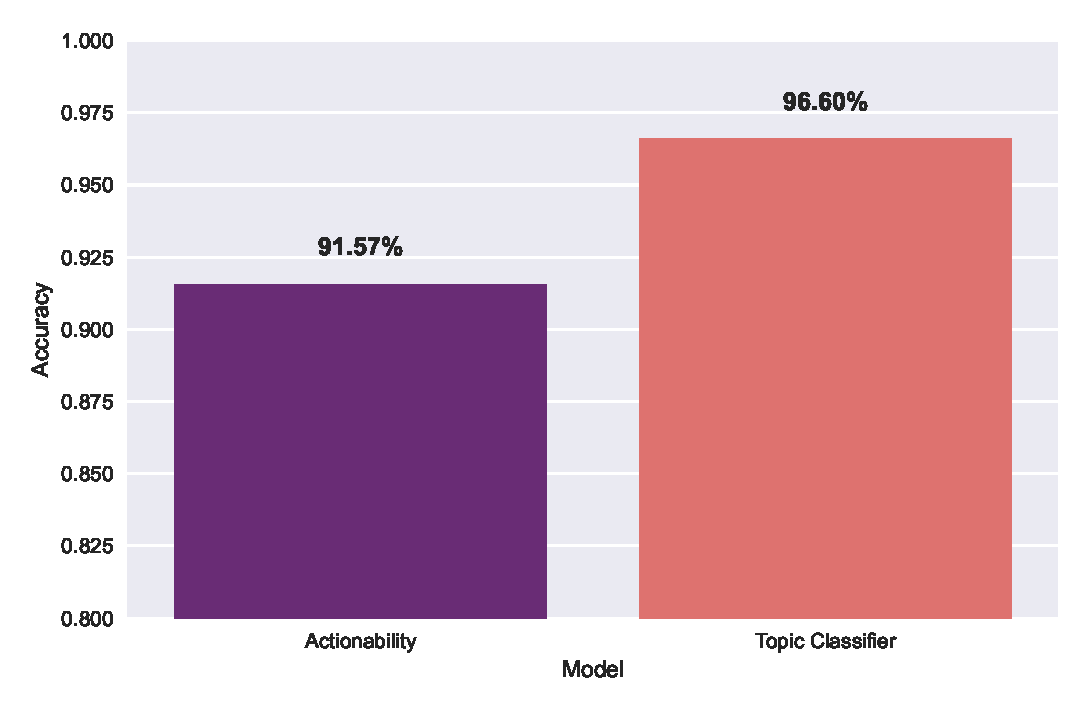
\includegraphics[width=0.8\textwidth]{figures/overall_accuracy.eps}
\caption{Overall accuracy of the ESG Topic Classifier and the Actionability Classifier on the Gold Set.}
\label{overall_accuracy}
\end{figure}

Beyond overall accuracy, class-level performance further confirms the robustness of the classification pipeline. As reported in Table~\ref{tab:classifier_performance}, the ESG Topic Classifier attains consistently high F1-scores across all thematic categories. For the Actionability Classifier, the Implemented and Indeterminate classes exhibit strong performance, while the Planning class remains more challenging (F1 = 0.52). This limitation reflects both the scarcity of labeled future-oriented commitments and the linguistic ambiguity between concrete plans and aspirational statements. Overall, the classification results provide reliable inputs for subsequent analytical stages.

\begin{table}
\centering
\caption{Performance of ESG Topic and Actionability Classifiers on the Gold Set.}
\label{tab:classifier_performance}
\begin{tabular}{llccc}
\hline
Task & Class & Precision & Recall & F1 \\
\hline
\multirow{6}{*}{ESG Topic}
& E (Environment) & 0.98 & 0.96 & 0.97 \\
& S\_labor & 0.98 & 0.97 & 0.98 \\
& S\_community & 0.96 & 0.98 & 0.97 \\
& S\_product & 0.95 & 0.96 & 0.95 \\
& G (Governance) & 0.96 & 0.94 & 0.95 \\
& Non-ESG & 0.94 & 0.96 & 0.95 \\
\hline
\multirow{3}{*}{Actionability}
& Implemented & 0.96 & 0.81 & 0.88 \\
& Planning & 0.59 & 0.46 & 0.52 \\
& Indeterminate & 0.93 & 0.96 & 0.95 \\
\hline
\end{tabular}
\end{table}

\subsection{Evidence Linking Evaluation}
The evidence linking module evaluates the system’s ability to retrieve internal support for ESG statements using a hybrid neuro–symbolic approach that combines rule-based pattern detection and semantic similarity modeling.

Empirical results indicate that 86.6\% of ESG statements are successfully linked to at least one supporting evidence sentence, with missing evidence concentrated among statements classified as Planning or Indeterminate. Compared with keyword-based baselines, the proposed approach achieves higher retrieval coverage, improved identification of implemented actions, and effective cross-sentence evidence linkage. These results highlight the advantage of semantic modeling over exact lexical matching in capturing substantively related ESG content (Fig.~\ref{evidence_method_comparison}).

\begin{figure}[!t]
\centering
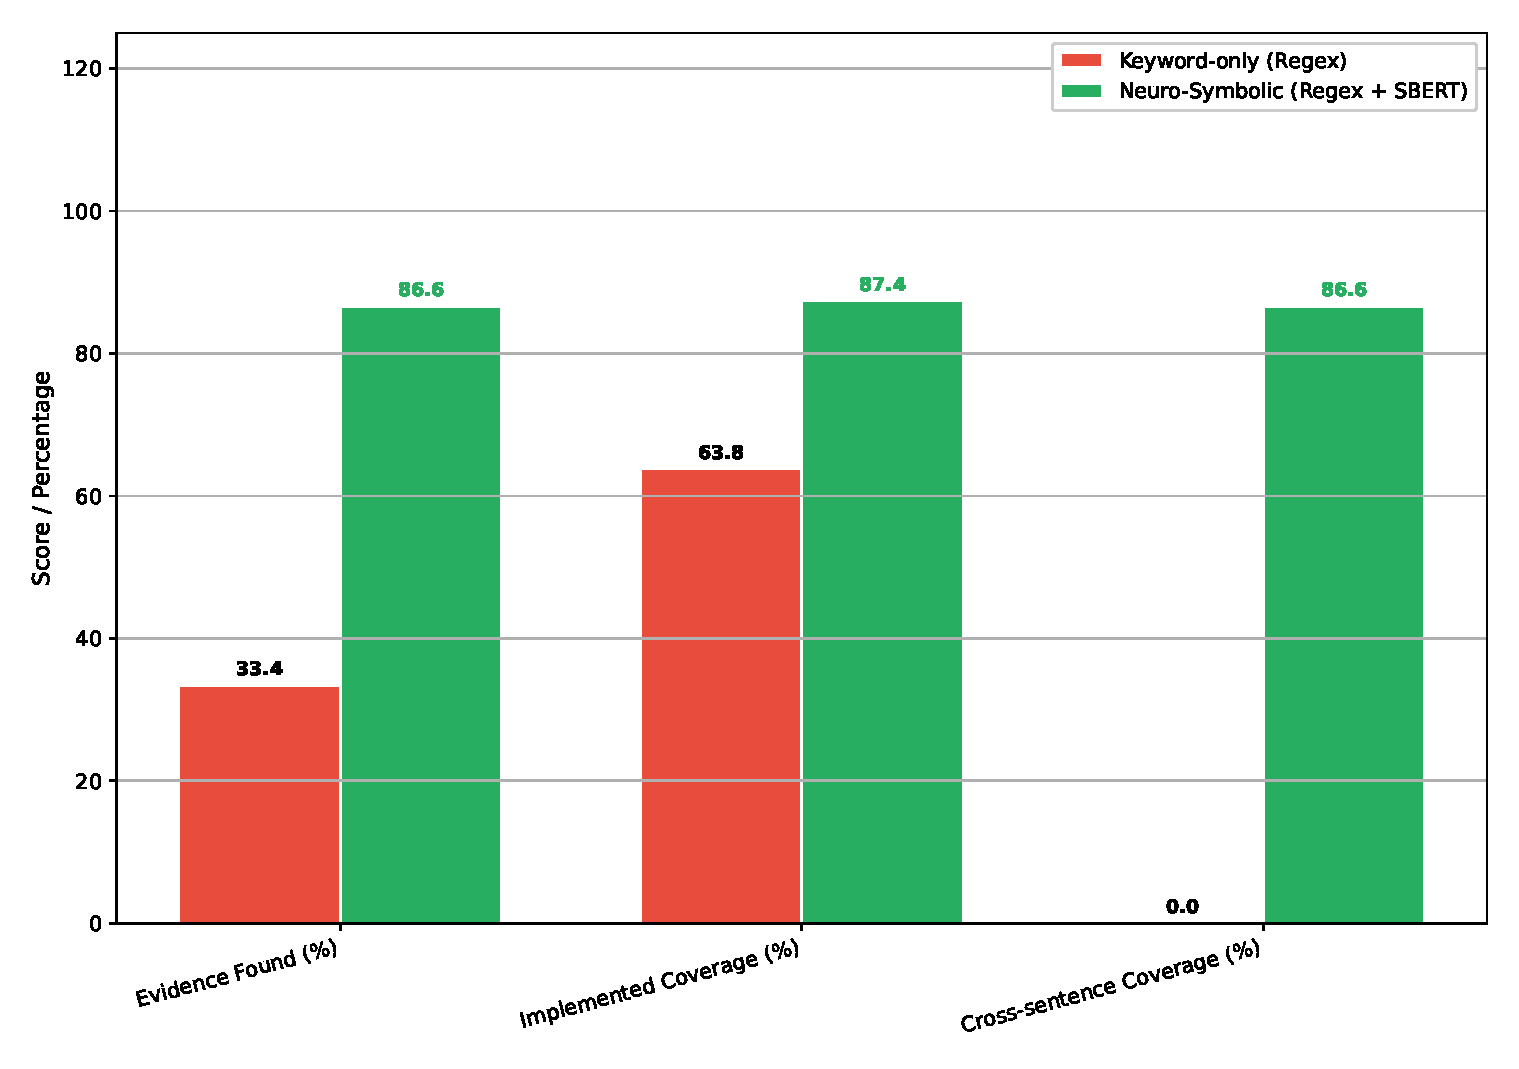
\includegraphics[width=0.8\textwidth]{figures/evidence_method_comparison.eps}
\caption{Comparison of evidence retrieval performance between keyword-based and neuro–symbolic approaches.}
\label{evidence_method_comparison}
\end{figure}

\subsection{ESG-Washing Risk Analysis}
Based on the ESG-Washing Risk Index (EWRI), the ESG-washing risk of annual reports from ten major Vietnamese banks is assessed (Fig.~\ref{ewri_rankings}). Substantial cross-bank variation is observed. Banks with higher EWRI values tend to rely more heavily on vague or weakly substantiated ESG statements, whereas lower-risk banks present clearer disclosures supported by concrete and verifiable evidence.

\begin{figure}[!t]
\centering
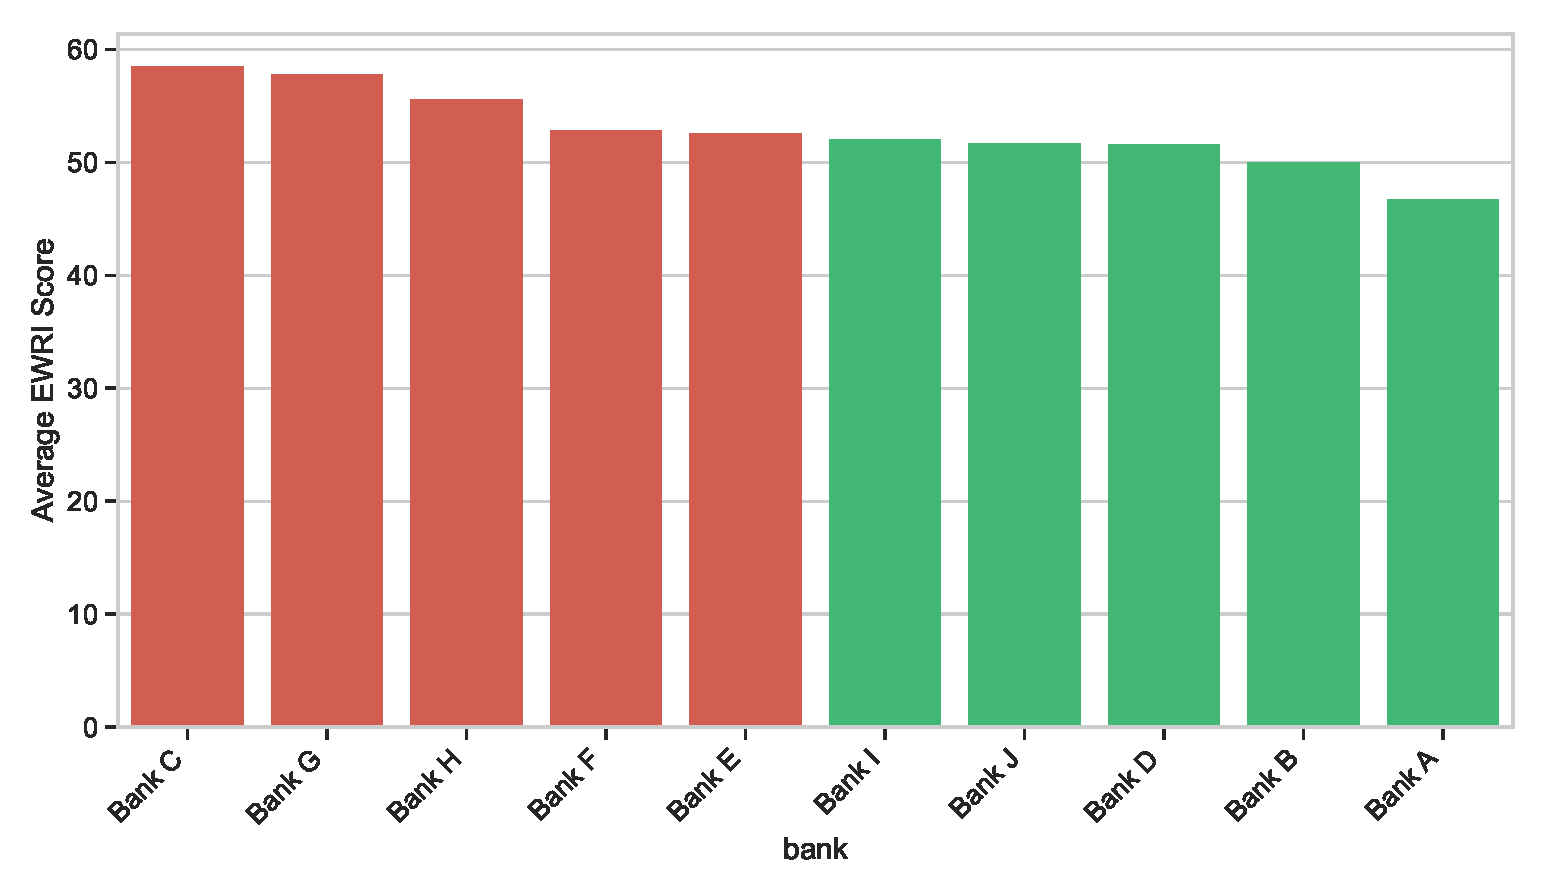
\includegraphics[width=0.8\textwidth]{figures/ewri_rankings.eps}
\caption{Comparison of ESG-washing risk scores across banks.}
\label{ewri_rankings}
\end{figure}

Temporal analysis reveals a clear dynamic pattern (Fig.~\ref{ewri_trend}). Average EWRI increases steadily and peaks in 2022, coinciding with a period of intensified commitment-oriented ESG communication, during which many banks announced Net Zero and sustainable finance goals without detailed implementation roadmaps. From 2023 onward, EWRI declines, reflecting a gradual shift toward more concrete, evidence-backed ESG disclosures.

\begin{figure}[!t]
\centering
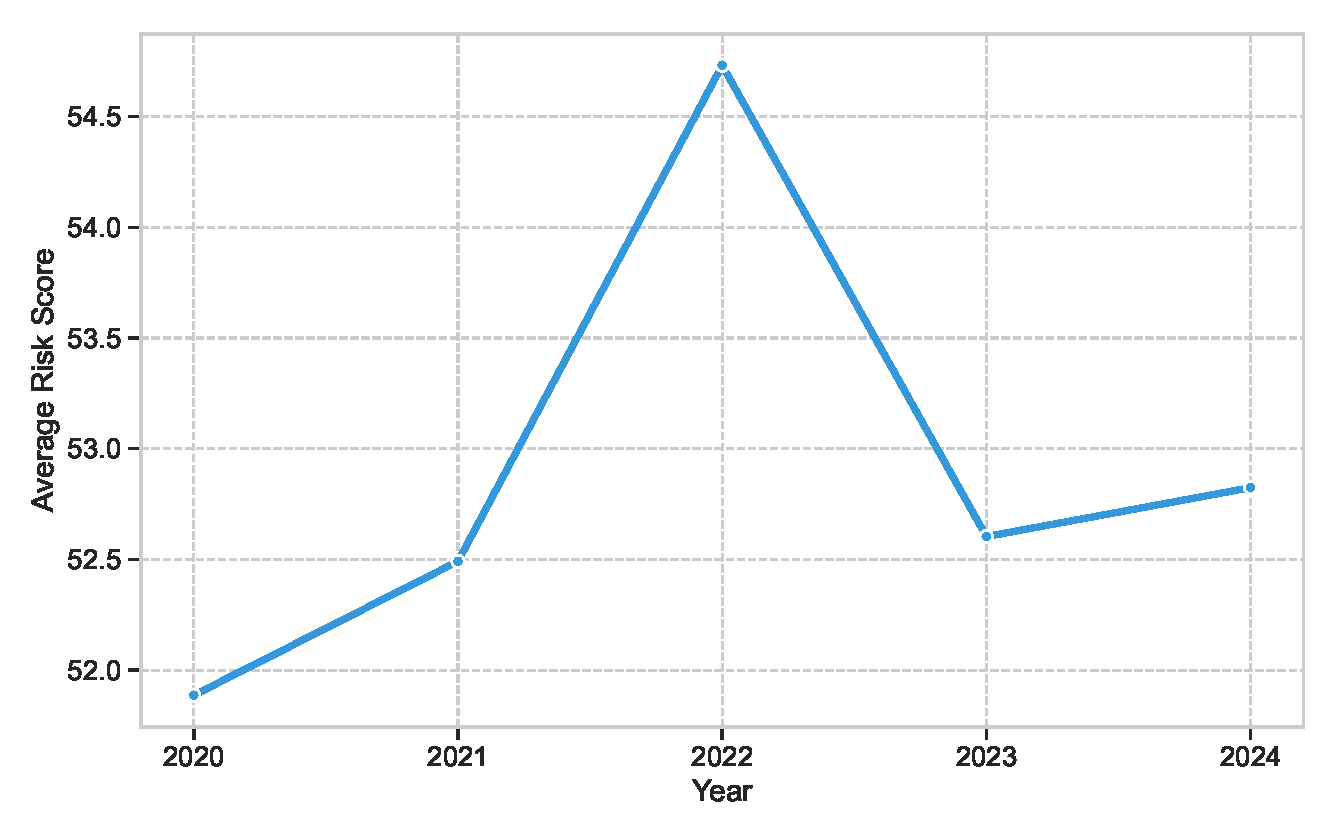
\includegraphics[width=0.8\textwidth]{figures/ewri_trend.eps}
\caption{Temporal trend of average EWRI scores from 2020 to 2024.}
\label{ewri_trend}
\end{figure}

\subsubsection{Correlation Analysis of EWRI Components}
Correlation analysis further validates the internal consistency of EWRI (Fig.~\ref{ablation_correlation}). The proportion of indeterminate statements exhibits a strong positive correlation with EWRI ($r = 0.977$), confirming that vague ESG commitments are a primary driver of ESG-washing risk. In contrast, average evidence strength and semantic similarity are negatively correlated with EWRI, indicating that stronger and more consistent evidence is associated with lower ESG-washing risk.

\begin{figure}[!t]
\centering
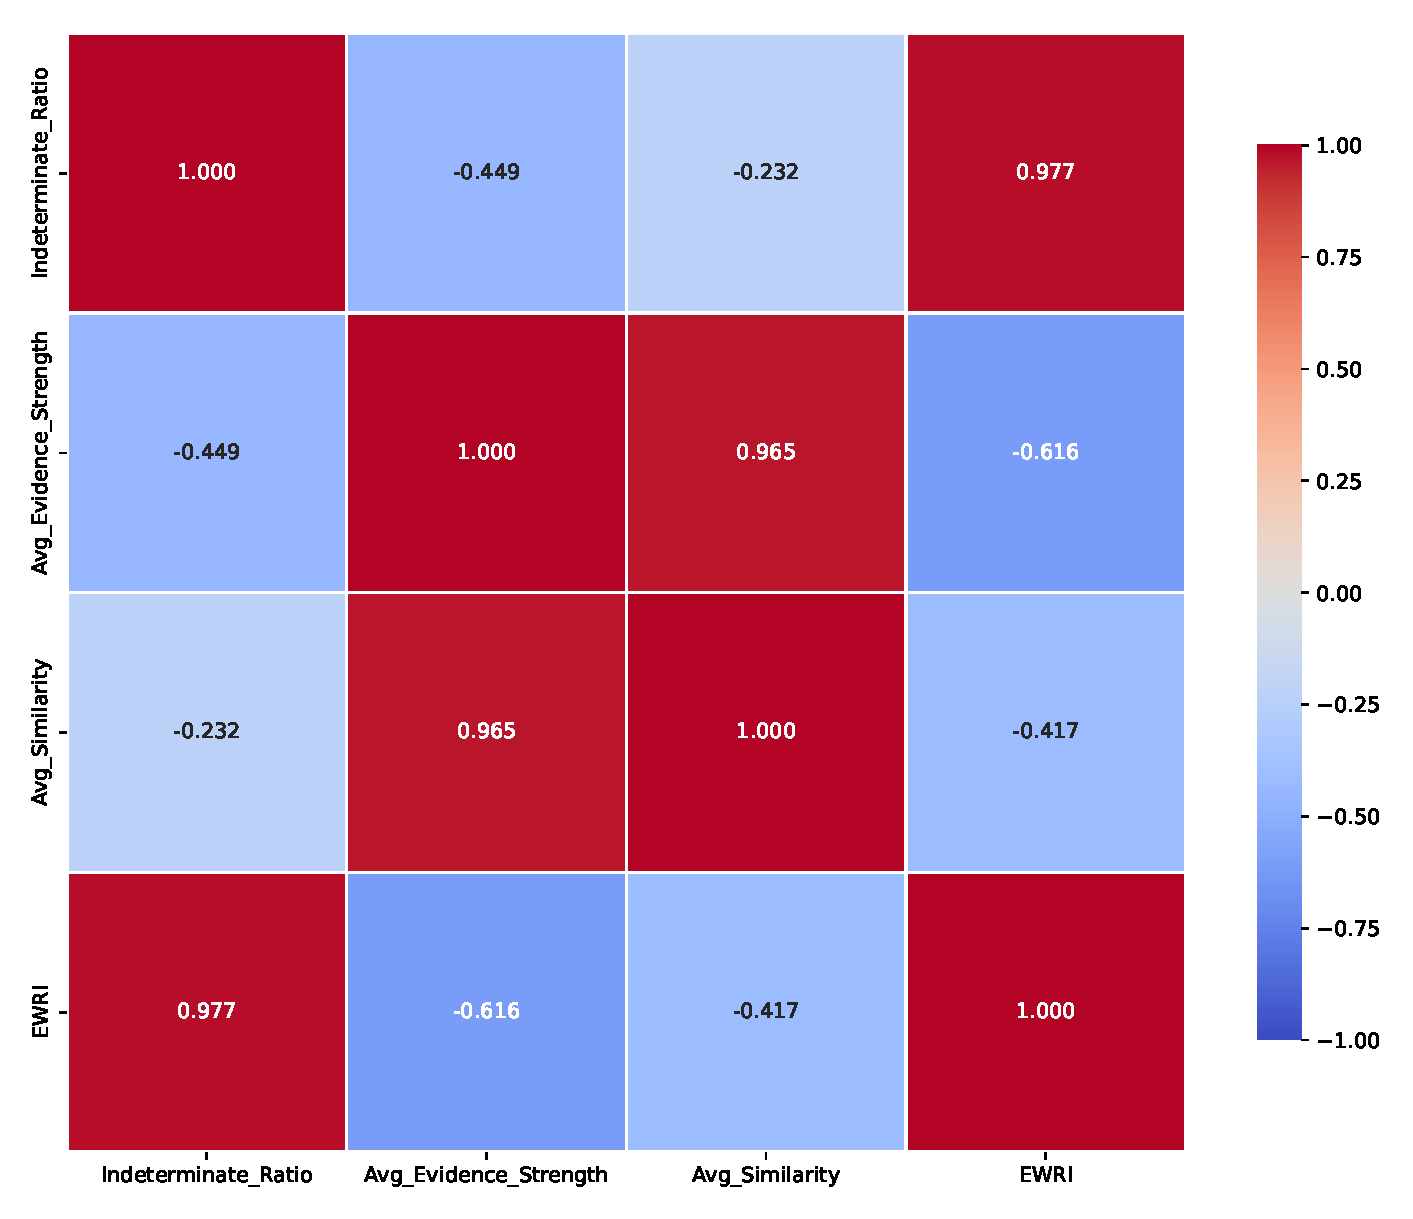
\includegraphics[width=0.8\textwidth]{figures/ablation_correlation.eps}
\caption{Correlation matrix of EWRI components.}
\label{ablation_correlation}
\end{figure}

A strong positive correlation between evidence strength and semantic similarity ($r = 0.965$) suggests that clearer and more specific ESG statements not only reduce ESG-washing risk but also facilitate more effective evidence retrieval (Fig.~\ref{ablation_scatter}).

\begin{figure}[!t]
\centering
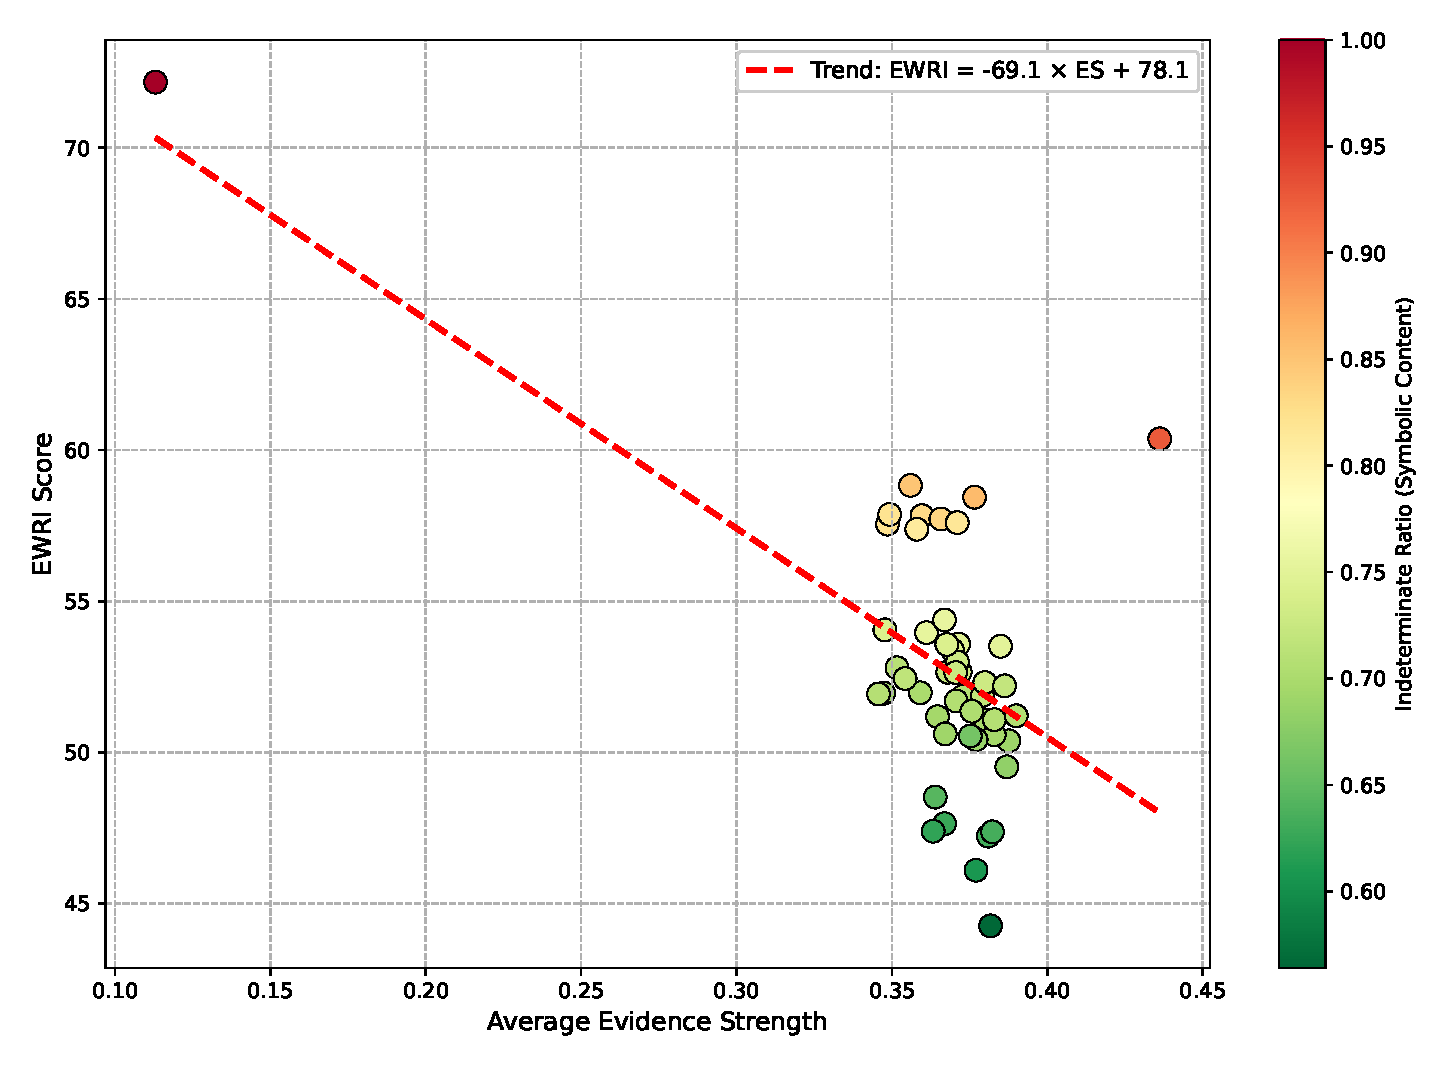
\includegraphics[width=0.8\textwidth]{figures/ablation_scatter.eps}
\caption{Relationship between Evidence Strength and EWRI.}
\label{ablation_scatter}
\end{figure}

%
%
%
\section{Conclusion}
This study proposes a neuro–symbolic NLP framework for assessing ESG-washing risk in the annual reports of Vietnamese commercial banks, with a focus on the internal verifiability of ESG disclosures. By integrating ESG topic classification, actionability assessment, and hybrid evidence linking, the framework introduces the ESG-Washing Risk Index (EWRI) as a quantitative measure of disclosure quality.

Experimental results demonstrate that the proposed approach effectively identifies vague and weakly substantiated ESG statements and outperforms keyword-based methods in evidence retrieval and interpretability. Application of EWRI to bank reports from 2020–2024 reveals substantial cross-bank variation in ESG-washing risk, as well as a clear temporal pattern in which risk peaks during periods of commitment-heavy ESG communication and declines as disclosures become more evidence-driven.

Overall, the findings suggest that improving the specificity and evidentiary grounding of ESG disclosures can mitigate ESG-washing risk without diminishing the communicative role of sustainability reporting. Future research may extend this framework by expanding annotated datasets and incorporating external information sources to further enhance robustness and generalizability.

\begin{credits}
\subsubsection{\discintname}
The authors have no competing interests to declare that are
relevant to the content of this article.
\end{credits}

%
% ---- Bibliography ----
\bibliographystyle{splncs04}
\bibliography{references}

\end{document}
